\chapter{CƠ SỞ LÝ THUYẾT VÀ CÔNG NGHỆ LIÊN QUAN}
\label{ch:chuong2}

\section{Tổng quan về Hệ thống IoT và Giao thức truyền thông}
\label{sec:tong_quan_iot}

\subsection{Kiến trúc IoT 5 tầng}
Internet of Things (IoT) là mô hình mạng kết nối vạn vật, cho phép các thiết bị vật lý thu thập, trao đổi dữ liệu và thực thi hành động điều khiển từ xa thông qua mạng Internet. Trong các hệ thống giám sát và quản lý thông minh quy mô lớn như tòa nhà hoặc ký túc xá, kiến trúc 5 tầng chuẩn hóa được áp dụng phổ biến nhằm phân tách rõ ràng trách nhiệm giữa các thành phần kỹ thuật:

\begin{enumerate}
    \item \textbf{Tầng cảm nhận (Perception/Sensing Layer):} Bao gồm các cảm biến vật lý (nhiệt độ, độ ẩm, khí gas) và thiết bị định danh (thẻ RFID) trực tiếp thu thập tín hiệu từ môi trường thực tế, cùng các cơ cấu chấp hành (relay điều khiển đèn, quạt, khóa từ, còi báo).
    \item \textbf{Tầng mạng và truyền thông (Network/Transport Layer):} Chịu trách nhiệm truyền dẫn an toàn dữ liệu từ các thiết bị ngoại vi tại phòng ở về trung tâm xử lý thông qua các giao thức mạng không dây (Wi-Fi 802.11 b/g/n) và các giao thức tầng ứng dụng tối ưu hóa băng thông như MQTT và WebSockets.
    \item \textbf{Tầng lưu trữ dữ liệu (Data Storage Layer):} Tiếp nhận, làm sạch và lưu trữ bền vững khối lượng lớn dữ liệu đo đạc cảm biến chuỗi thời gian (Time-Series Data) và dữ liệu quan hệ nghiệp vụ bằng hệ quản trị cơ sở dữ liệu PostgreSQL tích hợp TimescaleDB.
    \item \textbf{Tầng trí tuệ và xử lý ứng dụng (Application/Intelligence Layer):} Vận hành các mô hình học máy (Machine Learning) để dự báo phụ tải tiêu thụ điện, phát hiện sớm các bất thường vận hành của thiết bị, và thực thi các luật nghiệp vụ an toàn (Rule Engine).
    \item \textbf{Tầng trình diễn và quản trị nghiệp vụ (Presentation/Business Layer):} Cung cấp giao diện tương tác trực quan cho người dùng cuối (Dashboard quản trị cho cán bộ KTX và Cổng thông tin cá nhân hóa cho sinh viên nội trú).
\end{enumerate}

\subsection{Giao thức truyền thông MQTT}
Message Queuing Telemetry Transport (MQTT) là giao thức truyền thông điệp dạng xuất bản/đăng ký (Publish/Subscribe) cực kỳ gọn nhẹ, được chuẩn hóa bởi OASIS và thiết kế chuyên biệt cho các thiết bị nhúng có tài nguyên bộ nhớ và băng thông hạn chế.

\begin{figure}[H]
    \centering
    \begin{tikzpicture}[node distance=2.2cm, auto, >=stealth]
        \tikzstyle{block} = [rectangle, draw=blue!70, fill=blue!10, text width=2.8cm, text centered, rounded corners, minimum height=1.3cm, font=\small\bfseries]
        \tikzstyle{broker} = [rectangle, draw=red!70, fill=red!10, text width=3.2cm, text centered, rounded corners, minimum height=2.0cm, font=\small\bfseries]
        
        \node [block] (esp32) {ESP32 Edge Device\\(Publisher)};
        \node [broker, right=2.5cm of esp32] (broker) {MQTT Broker\\(Mosquitto)\\Topics Router};
        \node [block, above right=0.3cm and 2.5cm of broker] (backend) {NestJS Server\\(Subscriber / Pub)};
        \node [block, below right=0.3cm and 2.5cm of broker] (ai) {AI Service\\(Subscriber)};
        
        \draw [->, line width=1.2pt] (esp32) -- node[above, font=\footnotesize] {Publish telemetry} (broker);
        \draw [->, line width=1.2pt] (broker) -- node[above, sloped, font=\footnotesize] {Subscribe / Notify} (backend);
        \draw [->, line width=1.2pt] (broker) -- node[below, sloped, font=\footnotesize] {Subscribe stream} (ai);
        \draw [->, line width=1.2pt, dashed, red] (backend) -- node[below, font=\footnotesize] {Publish control} (broker);
        \draw [->, line width=1.2pt, dashed, red] (broker) -- node[below, font=\footnotesize] {Deliver command} (esp32);
    \end{tikzpicture}
    \caption{Mô hình truyền thông Publish/Subscribe thông qua MQTT Broker}
    \label{fig:mqtt_pub_sub}
\end{figure}

Giao thức MQTT hoạt động dựa trên các nguyên tắc then chốt:
\begin{itemize}
    \item \textbf{Định tuyến theo chủ đề (Topic-based Routing):} Thông điệp được gắn với một chuỗi ký tự phân cấp theo dấu gạch chéo, ví dụ: \texttt{smartdorm/rooms/A101/telemetry} hoặc \texttt{smartdorm/rooms/A101/commands}.
    \item \textbf{Chất lượng dịch vụ (Quality of Service - QoS):}
    \begin{itemize}
        \item \textit{QoS 0 (At most once):} Thông điệp được gửi tối đa 1 lần, không có gói tin phản hồi (ACK), chấp nhận khả năng mất tin nếu mạng chập chờn.
        \item \textit{QoS 1 (At least once):} Đảm bảo thông điệp được chuyển phát ít nhất 1 lần bằng cơ chế bắt tay hai chiều (PUBACK). Đây là mức QoS được lựa chọn triển khai trong SmartDorm để đảm bảo các dữ liệu cảm biến khẩn cấp và lệnh điều khiển relay không bị thất lạc.
        \item \textit{QoS 2 (Exactly once):} Đảm bảo thông điệp chỉ được nhận duy nhất 1 lần qua quy trình bắt tay 4 bước (PUBREC, PUBREL, PUBCOMP), có độ trễ lớn hơn.
    \end{itemize}
    \item \textbf{Gói tin giữ kết nối (Keep-Alive) và Di chúc (Last Will and Testament - LWT):} Cho phép máy chủ phát hiện ngay lập tức tình trạng vi điều khiển tại phòng bị mất nguồn hoặc ngắt kết nối mạng bất ngờ, từ đó tự động phát sinh cảnh báo Offline trên giao diện quản trị.
\end{itemize}

\subsection{Giao thức WebSockets và Socket.io}
Khác với giao thức HTTP truyền thống vận hành theo mô hình yêu cầu/phản hồi (Request/Response) đơn hướng gây hao phí tiêu đề gói tin (overhead) khi thực hiện cơ chế thăm dò định kỳ (polling), WebSockets cung cấp một kênh giao tiếp hai chiều (Full-Duplex) liên tục qua một kết nối TCP duy nhất sau giai đoạn bắt tay ban đầu (Handshake). Thư viện Socket.io được tích hợp tại máy chủ NestJS cho phép đẩy (push) dữ liệu đo đạc mới nhất từ tầng Backend xuống các trình duyệt Web phía Client với độ trễ dưới $20\text{ms}$, mang lại trải nghiệm cập nhật tức thì đồ thị cảm biến và trạng thái chuyển mạch thiết bị mà không cần tải lại trang.

\section{Phần cứng nhúng và Cảm biến môi trường}
\label{sec:phan_cung_va_cam_bien}

\subsection{Vi điều khiển trung tâm ESP32 DevKit V1}
ESP32 là hệ thống vi mạch trên một chip (System on a Chip - SoC) tiên tiến do hãng Espressif Systems phát triển, được trang bị bộ vi xử lý lõi kép 32-bit Xtensa LX6 với tần số xung nhịp lên đến $240\text{ MHz}$, bộ nhớ RAM nội bộ $520\text{ KB}$, cùng khả năng tích hợp sẵn Wi-Fi chuẩn $802.11\text{ b/g/n}$ và Bluetooth v4.2 BR/EDR \& BLE.

\begin{figure}[H]
    \centering
    \begin{tabular}{cc}
        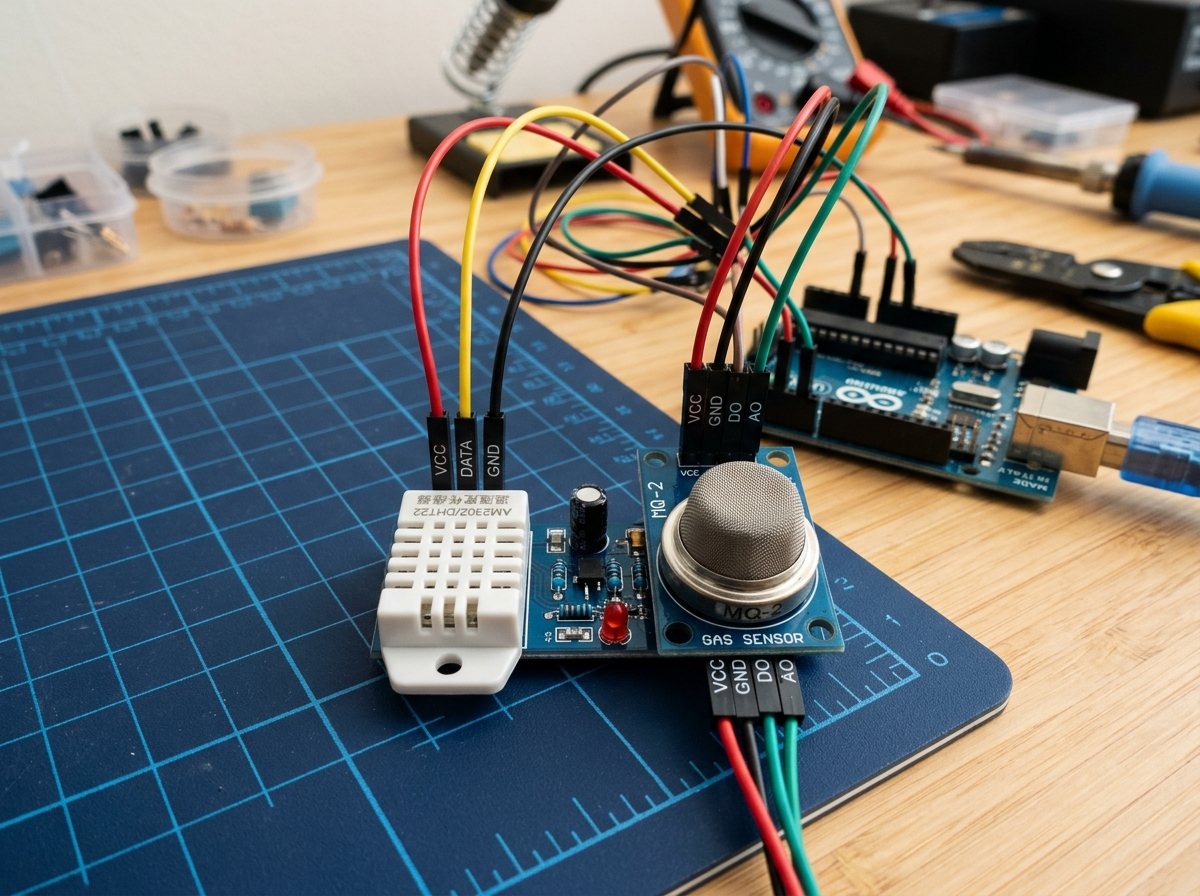
\includegraphics[width=0.45\textwidth]{figures/cam_bien_dht22_mq2.jpg} &
        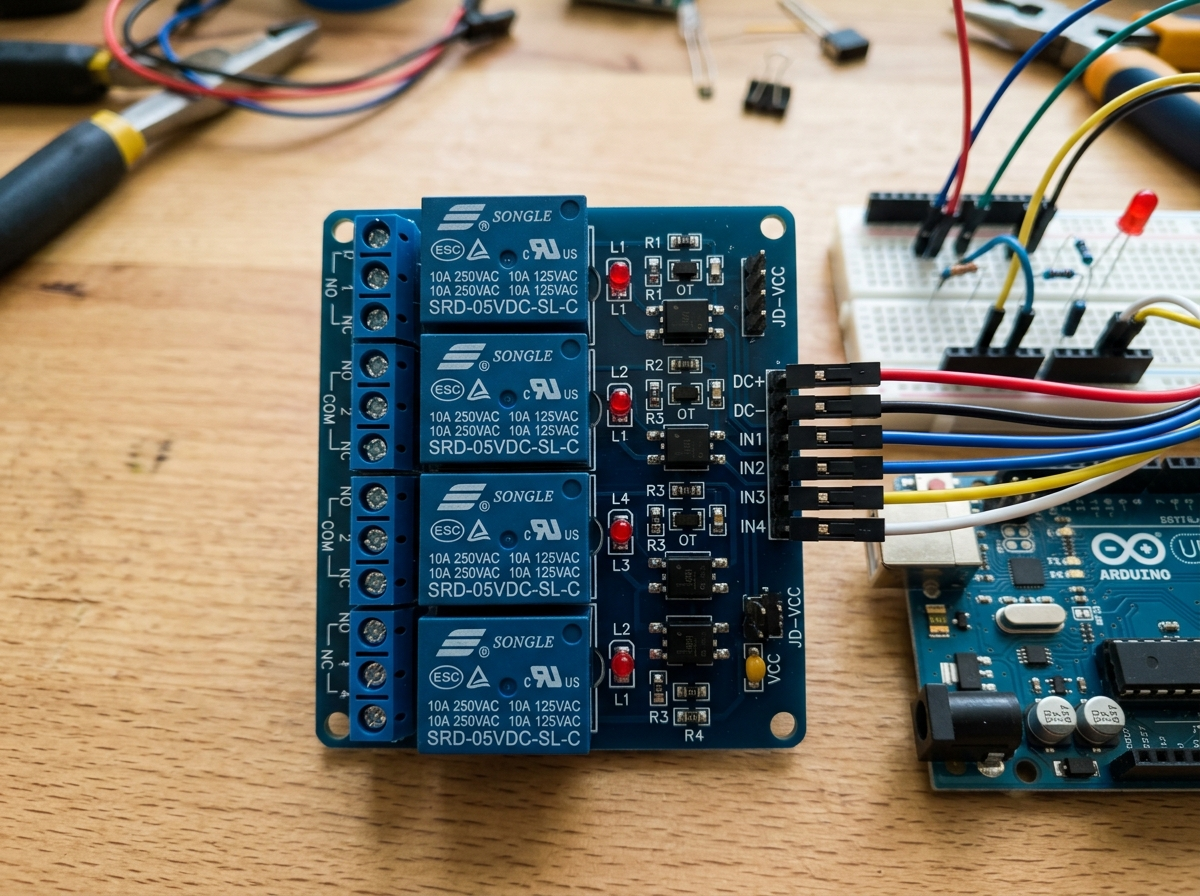
\includegraphics[width=0.45\textwidth]{figures/module_relay_4kenh.jpg} \\
        \small (a) Cảm biến DHT22 và MQ-2 & \small (b) Module Relay 4 kênh cách ly quang \\[0.3cm]
        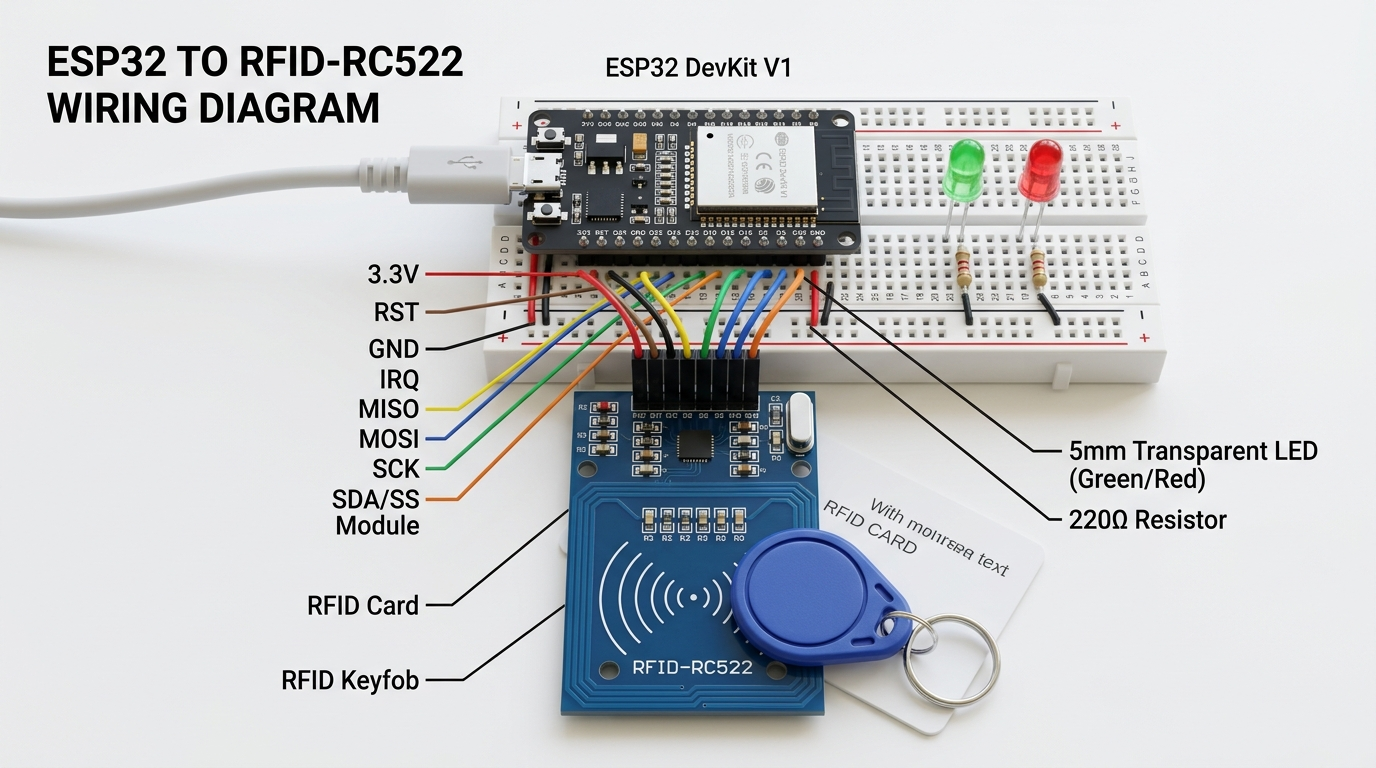
\includegraphics[width=0.45\textwidth]{figures/rfid_led_wiring.jpg} &
        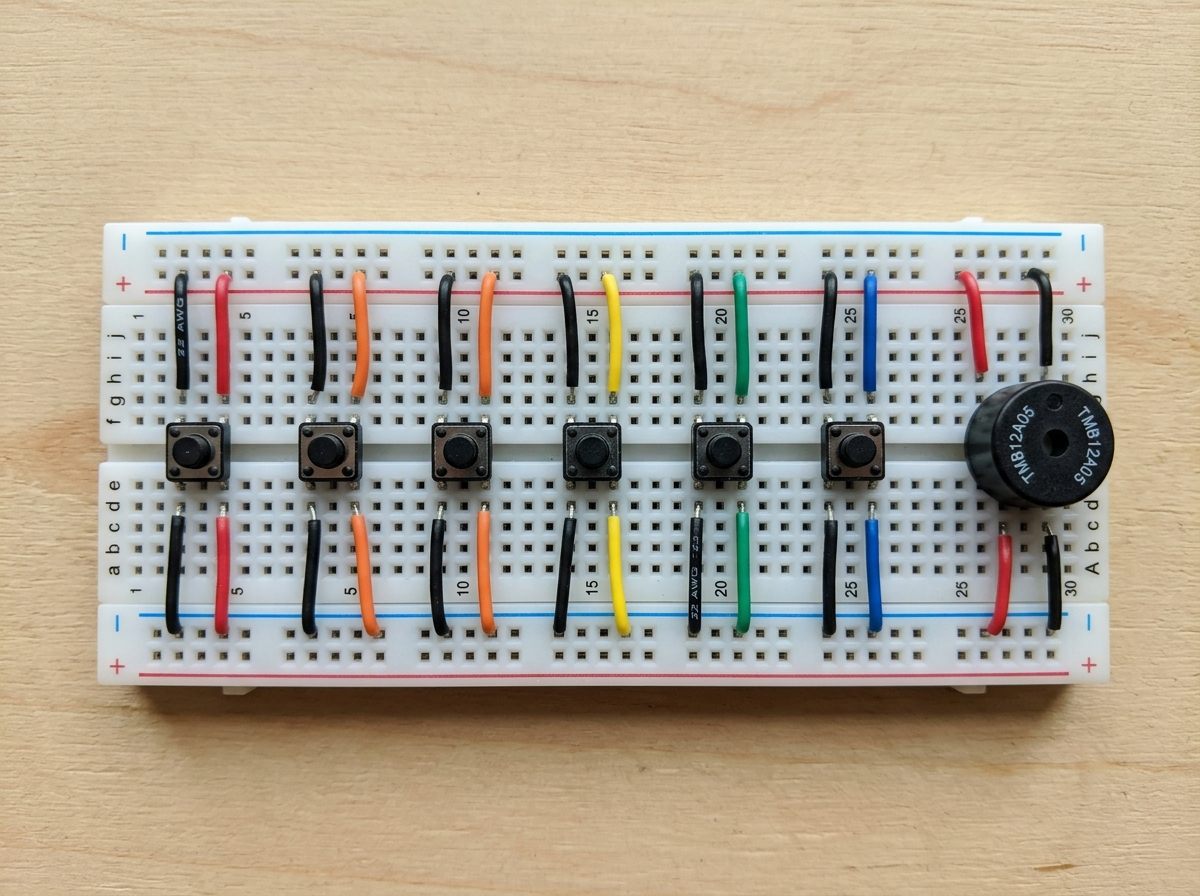
\includegraphics[width=0.45\textwidth]{figures/nut_nhan_va_coi.jpg} \\
        \small (c) Đấu dây đầu đọc RFID RC522 & \small (d) Nút nhấn điều khiển và Còi Buzzer
    \end{tabular}
    \caption{Các linh kiện phần cứng nhúng thực tế của hệ thống SmartDorm}
    \label{fig:hardware_components}
\end{figure}

ESP32 sở hữu các khối ngoại vi phần cứng phong phú rất phù hợp cho các ứng dụng IoT tòa nhà:
\begin{itemize}
    \item Bộ chuyển đổi tương tự - số (ADC) 12-bit (với 18 kênh đầu vào, độ phân giải giá trị từ $0 \div 4095$).
    \item Các chuẩn giao tiếp phần cứng tốc độ cao: SPI (Serial Peripheral Interface), I2C, UART, PWM.
    \item Hỗ trợ hệ điều hành thời gian thực FreeRTOS đa nhiệm (Multitasking), cho phép phân bổ riêng biệt tác vụ đọc cảm biến chu kỳ trên một lõi (Core 0) và tác vụ duy trì kết nối mạng Wi-Fi/MQTT trên lõi còn lại (Core 1).
\end{itemize}

\subsection{Cảm biến nhiệt độ và độ ẩm DHT22 (AM2302)}
DHT22 là cảm biến kỹ thuật số tích hợp khối đo độ ẩm bằng vật liệu điện dung (Capacitive Humidity Sensor) và khối đo nhiệt độ bằng điện trở nhiệt NTC (Negative Temperature Coefficient thermistor). Cảm biến có bộ vi điều khiển 8-bit tích hợp bên trong để thực hiện việc chuyển đổi tín hiệu tương tự sang chuỗi dữ liệu nhị phân 40-bit và truyền về ESP32 qua giao thức 1 dây (One-Wire) tại chân GPIO 4:
\begin{itemize}
    \item Dải đo nhiệt độ: $-40^\circ\text{C} \div +80^\circ\text{C}$ với độ chính xác cao $\pm 0.5^\circ\text{C}$.
    \item Dải đo độ ẩm: $0\% \div 100\%\text{ RH}$ với sai số $\pm 2\%\text{ RH}$.
    \item Tần suất lấy mẫu: $0.5\text{ Hz}$ (2 giây một lần), đảm bảo tính ổn định và tránh hiện tượng tự sinh nhiệt của cảm biến.
\end{itemize}

\subsection{Cảm biến khí gas và khói MQ-2}
MQ-2 là cảm biến khí bán dẫn sử dụng màng cảm biến thiếc đioxit ($\text{SnO}_2$). Khi đặt trong không khí sạch, độ dẫn điện của cảm biến ở mức thấp; khi tiếp xúc với các loại khí dễ cháy như khí dầu mỏ hóa lỏng (LPG), Propane, Methane, khói hoặc cồn sinh học, độ dẫn điện của cảm biến sẽ tăng tỷ lệ thuận với nồng độ khí trong môi trường.

Tín hiệu điện áp ngõ ra tương tự (Analog Output) của module cảm biến MQ-2 được đưa vào chân GPIO 34 của ESP32. Chân GPIO 34 là chân đầu vào ADC chuyên dụng (Input-only, không có điện trở kéo nội) giúp triệt tiêu hoàn toàn hiện tượng nhiễu xung số. Giá trị ADC đo được ($ADC_{val} \in [0, 4095]$) được chuyển đổi thành phần trăm nồng độ chuẩn hóa theo công thức:
\begin{equation}
    Gas_{pct} = \left(\frac{ADC_{val}}{4095}\right) \times 100\%
    \label{eq:gas_conversion}
\end{equation}

\subsection{Đầu đọc thẻ thông minh RFID RC522}
Module RC522 dựa trên chip truyền thông không tiếp xúc MFRC522 của NXP Semiconductors, hoạt động ở dải tần vô tuyến cao $13.56\text{ MHz}$ theo tiêu chuẩn ISO/IEC 14443A. Thiết bị giao tiếp với vi điều khiển ESP32 thông qua bus giao tiếp ngoại vi nối tiếp đồng bộ SPI (Serial Peripheral Interface) tốc độ cao với 4 đường tín hiệu chính:
\begin{itemize}
    \item SCK (Serial Clock) kết nối GPIO 18.
    \item MOSI (Master Out Slave In) kết nối GPIO 23.
    \item MISO (Master In Slave Out) kết nối GPIO 19.
    \item SDA/SS (Slave Select) kết nối GPIO 5; cùng chân RST (Reset) kết nối GPIO 22.
\end{itemize}
Khi sinh viên đưa thẻ từ (Mifare Classic 1K) vào vùng từ trường bức xạ anten của module (khoảng cách $0 \div 5\text{ cm}$), chíp trên thẻ được cấp nguồn cảm ứng điện từ và phản hồi mã định danh duy nhất (Unique Identifier - UID) dạng chuỗi Hex. Firmware ESP32 đọc mã này và gửi ngay gói tin MQTT về máy chủ Backend để kiểm tra phân quyền mở cửa.

\subsection{Module Relay 4 kênh cách ly quang và Thiết bị báo động}
Module Relay 4 kênh chịu tải điện áp tối đa $250\text{V AC} / 10\text{A}$ hoặc $30\text{V DC} / 10\text{A}$. Nhằm bảo vệ an toàn tuyệt đối cho vi điều khiển ESP32 trước các xung điện áp cảm ứng ngược và hiện tượng nhiễu từ trường khi đóng cắt cuộn hút, module sử dụng các linh kiện cách ly quang (Optocoupler EL817) phân tách độc lập giữa mạch điều khiển logic $3.3\text{V}$ và nguồn kích cuộn hút $5\text{V}$. Các chân kích hoạt Relay kết nối với các ngõ ra GPIO 25 (Đèn), GPIO 14 (Quạt), GPIO 12 (Điều hòa) và GPIO 13 (Khóa từ). Thiết bị sử dụng logic kích hoạt mức thấp (Active-LOW trigger).

Còi báo động Buzzer Active ($5\text{V}$) kết nối với chân GPIO 15, cho phép phát ra âm thanh cảnh báo decibel cao khi nồng độ khí gas vượt ngưỡng cho phép, ngay cả trong trường hợp mất kết nối mạng Internet.

\section{Cơ sở lý thuyết Học máy (Machine Learning)}
\label{sec:ly_thuyet_hoc_may}

\subsection{Thuật toán Gradient Boosting Regressor (GBM) với Huber Loss}
Trong bài toán dự báo phụ tải tiêu thụ điện năng của ký túc xá, dữ liệu đo đạc thực tế thường chứa nhiều điểm bất thường và đột biến (outliers) do sinh viên đột xuất sử dụng các thiết bị công suất cao vào mùa thi cử hoặc thay đổi thời gian sinh hoạt vào các dịp lễ. Việc sử dụng các hàm tổn thất bình phương trung bình cổ điển ($L_2$ Loss / MSE) thường khiến mô hình bị lệch nghiêm trọng do phạt quá nặng các điểm đột biến này (bậc 2 của sai số).

Để khắc phục hiện tượng trên, đề tài áp dụng mô hình cây tăng cường độ dốc \textbf{Gradient Boosting Machine (GBM)} kết hợp với \textbf{Hàm tổn thất Huber (Huber Loss)}.

\subsubsection{Cơ chế tăng cường độ dốc (Gradient Boosting)}
Mô hình Gradient Boosting xây dựng chuỗi các cây quyết định cơ sở (Weak Learners) $h_m(x)$ theo phương pháp cộng dồn từng bước (Forward Stagewise Additive Modeling):
\begin{equation}
    F_m(x) = F_{m-1}(x) + \gamma_m h_m(x)
    \label{eq:gbm_update}
\end{equation}
Trong đó tại mỗi vòng lặp thứ $m$, mô hình sẽ khớp một cây quyết định mới $h_m(x)$ vào phần thặng dư giả định (Pseudo-residuals), bản chất là gradient âm của hàm tổn thất $L(y, F(x))$ đối với giá trị dự báo ở bước trước:
\begin{equation}
    r_{im} = -\left[ \frac{\partial L(y_i, F(x_i))}{\partial F(x_i)} \right]_{F(x) = F_{m-1}(x)}
    \label{eq:gbm_residuals}
\end{equation}

\subsubsection{Hàm tổn thất Huber (Huber Loss Function)}
Hàm tổn thất Huber là sự dung hòa tối ưu giữa hàm bình phương sai số $L_2$ (khi độ lệch nhỏ hơn ngưỡng $\delta$) và hàm sai số tuyệt đối $L_1$ (khi độ lệch lớn hơn ngưỡng $\delta$), được định nghĩa toán học như sau:
\begin{equation}
    L_\delta(y, F(x)) = 
    \begin{cases} 
        \frac{1}{2} (y - F(x))^2 & \text{với } |y - F(x)| \le \delta \\[0.2cm]
        \delta |y - F(x)| - \frac{1}{2} \delta^2 & \text{với } |y - F(x)| > \delta 
    \end{cases}
    \label{eq:huber_loss}
\end{equation}
Đạo hàm của hàm tổn thất Huber theo giá trị dự báo $F(x)$ có dạng:
\begin{equation}
    \frac{\partial L_\delta(y, F(x))}{\partial F(x)} = 
    \begin{cases} 
        -(y - F(x)) & \text{với } |y - F(x)| \le \delta \\[0.2cm]
        -\delta \cdot \text{sgn}(y - F(x)) & \text{với } |y - F(x)| > \delta 
    \end{cases}
    \label{eq:huber_derivative}
\end{equation}
Nhờ đặc tính đạo hàm bị chặn bởi $[-\delta, \delta]$ khi sai số lớn, Gradient Boosting sử dụng Huber Loss loại bỏ hoàn toàn hiện tượng bùng nổ gradient khi gặp dữ liệu nhiễu hoặc đột biến phụ tải, giúp mô hình hội tụ ổn định và đạt độ chính xác dự báo vượt trội.

\subsection{Thuật toán Rừng cô lập (Isolation Forest)}
Để phát hiện sớm các thiết bị điện sinh hoạt trong phòng có dấu hiệu hư hỏng, rò điện hoặc bị sinh viên cắm điện liên tục không giám sát, thuật toán \textbf{Isolation Forest (iForest)} được triển khai.

Khác với các phương pháp phát hiện bất thường truyền thống dựa trên việc mô hình hóa vùng mật độ bình thường (như One-Class SVM hay k-NN) vốn đòi hỏi chi phí tính toán cao, Isolation Forest dựa trên một quan sát thực nghiệm sâu sắc: \textit{Các điểm dữ liệu bất thường (Anomalies) thường có số lượng rất ít và mang các giá trị đặc trưng khác biệt đáng kể so với đại đa số, do đó chúng rất dễ bị cô lập chỉ sau một vài lát cắt ngẫu nhiên trong không gian đặc trưng.}

Thuật toán xây dựng một tập hợp các cây cô lập (Isolation Trees - iTree). Tại mỗi nút phân nhánh của iTree, thuật toán chọn ngẫu nhiên một đặc trưng $q$ và chọn ngẫu nhiên một giá trị ngưỡng cắt $p$ nằm giữa giá trị cực tiểu và cực đại của đặc trưng đó trong tập con dữ liệu hiện tại.

Độ dài đường dẫn $h(x)$ là số lượng cạnh mà điểm dữ liệu $x$ phải đi qua từ gốc của cây cho đến khi rơi vào một nút lá cô lập. Điểm bất thường (Anomaly Score) $s(x, n)$ của mẫu dữ liệu $x$ đối với tập dữ liệu có quy mô $n$ mẫu được định chuẩn theo công thức:
\begin{equation}
    s(x, n) = 2^{-\frac{E(h(x))}{c(n)}}
    \label{eq:isolation_score}
\end{equation}
Trong đó $E(h(x))$ là độ dài đường dẫn trung bình của $x$ qua toàn bộ các cây cô lập trong rừng; $c(n)$ là độ dài đường dẫn trung bình lý thuyết của một cây tìm kiếm nhị phân không thành công chứa $n$ nút:
\begin{equation}
    c(n) = 2 \ln(n - 1) + 0.5772156649 \text{ (hằng số Euler-Mascheroni)} - \frac{2(n - 1)}{n}
    \label{eq:euler_constant}
\end{equation}
Đánh giá giá trị điểm số bất thường $s(x, n) \in [0, 1]$:
\begin{itemize}
    \item Nếu $s(x, n) \to 1$ ($E(h(x)) \ll c(n)$): Điểm dữ liệu bị cô lập rất nhanh gần gốc cây $\rightarrow$ Khả năng rất cao là \textbf{bất thường}.
    \item Nếu $s(x, n) < 0.5$ ($E(h(x)) \ge c(n)$): Điểm dữ liệu nằm sâu trong tán cây $\rightarrow$ Dữ liệu \textbf{hoàn toàn bình thường}.
\end{itemize}

\section{Công nghệ phần mềm và Nền tảng phát triển}
\label{sec:cong_nghe_phan_mem}

\subsection{Nền tảng máy chủ NestJS}
NestJS là framework Node.js mã nguồn mở tiến tiến viết bằng ngôn ngữ TypeScript, được xây dựng dựa trên kiến trúc phân tầng vững chắc (Layered Architecture) tương tự Spring Boot trong Java hay Angular ở Frontend. NestJS áp dụng triệt để nguyên lý Đảo ngược phụ thuộc (Inversion of Control - IoC) và Tiêm phụ thuộc (Dependency Injection - DI), chia ứng dụng thành các Mô-đun (Modules), Bộ điều khiển (Controllers), Dịch vụ nghiệp vụ (Services) và Cổng kết nối thời gian thực (Gateways).

\subsection{Nền tảng giao diện Next.js 16}
Next.js 16 là framework React hàng đầu hiện nay, ứng dụng kiến trúc App Router tân tiến cùng cơ chế React Server Components (RSC). Next.js cho phép hiển thị trước mã HTML tại máy chủ (Server-Side Rendering - SSR) giúp cải thiện tối đa tốc độ tải trang ban đầu (First Contentful Paint - FCP), đồng thời kết hợp linh hoạt cơ chế Client-Side Rendering (CSR) để xử lý các bảng điều khiển động, nhận luồng dữ liệu WebSocket từ cảm biến và vẽ biểu đồ Recharts tương tác mượt mà.

\subsection{Cơ sở dữ liệu PostgreSQL, TimescaleDB và Prisma ORM}
\begin{itemize}
    \item \textbf{PostgreSQL:} Hệ quản trị cơ sở dữ liệu quan hệ đối tượng mạnh mẽ, tuân thủ nghiêm ngặt các tính chất toàn vẹn dữ liệu ACID (Atomicity, Consistency, Isolation, Durability).
    \item \textbf{TimescaleDB:} Phần mở rộng (Extension) chuyên dụng của PostgreSQL tối ưu cho chuỗi thời gian, tự động phân vùng bảng lớn thành các khối dữ liệu nhỏ theo thời gian (Hypertables), giúp tăng tốc độ truy vấn số liệu cảm biến lên gấp hàng chục lần so với bảng quan hệ thông thường.
    \item \textbf{Prisma ORM:} Bộ công cụ ánh xạ đối tượng hiện đại dành cho TypeScript, cung cấp khả năng tạo mô hình dữ liệu khai báo (\texttt{schema.prisma}), tự động sinh mã Migration cơ sở dữ liệu an toàn và hỗ trợ kiểm tra kiểu dữ liệu tĩnh (Type-safe Queries) tại thời điểm biên dịch.
\end{itemize}

\subsection{Dịch vụ Trí tuệ nhân tạo FastAPI}
FastAPI là framework web Python hiệu năng cao phát triển trên nền tảng Starlette và Pydantic, hỗ trợ lập trình bất đồng bộ chuẩn \texttt{async/await} nguyên bản. FastAPI đóng vai trò là microservice chuyên biệt đảm nhận nhiệm vụ nạp mô hình học máy đã được huấn luyện sẵn (Scikit-learn, XGBoost), trích xuất 13 đặc trưng đầu vào và phản hồi kết quả suy luận dự báo phụ tải với độ trễ siêu thấp dưới $15\text{ms}$.
\newpage
